\documentclass[11pt,a4paper]{article}

\usepackage[T1]{fontenc}

\usepackage{lmodern}
\usepackage{microtype}
\usepackage[a4paper,margin=2.6cm]{geometry}
\usepackage{amsmath}
\usepackage{booktabs}
\usepackage{eurosym}
\usepackage{enumitem}
\usepackage{caption}
\usepackage{pgfplots}
\pgfplotsset{compat=1.18}
\usepackage[numbers,sort&compress]{natbib}
\usepackage[hidelinks]{hyperref}

\captionsetup{font=small,labelfont=bf}
\setlist{itemsep=2pt,topsep=4pt}
\newcommand{\eur}[1]{\euro{}#1}

% Live counters from https://miles.bolls.dev/ops/api/health (.tabpfn), fetched at \livets.
\newcommand{\livets}{2026-11-22 08:56 UTC}
\newcommand{\livecalls}{298}
\newcommand{\liveok}{294}
\newcommand{\livefallbackbatches}{4}
\newcommand{\liverowstabpfn}{8{,}129}
\newcommand{\liverowsfallback}{72}
\newcommand{\livepfifty}{1.56}
\newcommand{\livepninety}{2.45}

\title{\textbf{Rescue before it strands:}\\[2pt]
Per-ride stranding prediction and incentive-based relocation\\
for free-floating car sharing with a tabular foundation model\thanks{Code, data processing and this paper's source: \url{https://github.com/LinusBolls/miles-ahead}.}}
\author{Linus Bolls \and Carolina Blasco}
\date{Prior Labs HACKLAB \#2, Berlin, 22 November 2026\\[4pt]
\small Open-source applied-research proof of concept. Unofficial; not affiliated with MILES.}

\begin{document}
\maketitle

\begin{abstract}
\noindent In free-floating car sharing a car can end a rental in a place where nobody wants it next. In Berlin in June 2024, about 2,700 ride ends per day (18\%) were followed by more than 12 hours idle. These cars are not broken: 88\% of such waits end in a normal booking or ride and 0.1\% in a repair. They are in the wrong place. The operator, MILES, relocates about 180 cars per day, starting a median 24.6\,h after the last customer ride. We ask whether stranding can be predicted at the moment a ride ends, so that a nearby user can be paid a small credit to move the car before the day is lost. We use TabPFN, a tabular foundation model, with a fixed 10,000-row context and no tuning, and compare it with gradient-boosted trees (GBM) and logistic regression on a strict time split (train 3--16 June 2024, test 17--22 June). TabPFN reaches AUC 0.846 (ECE 0.010) on 5\% of the training data. A GBM trained on all 208k rows still has the highest accuracy (AUC 0.858, ECE 0.008); at the same 10k-row budget the GBM reaches 0.825 with three times the calibration error (0.030). In a new city, with Berlin rides as context and no training, TabPFN reaches AUC 0.665 to 0.710 as local rides grow from 50 to 1,000; a GBM trained on Berlin alone stays flat at about 0.65. The same model family gives a value map of where a moved car will be rented soonest (AUC 0.777) and a still-there probability that prices a money-back guarantee (AUC 0.827; 4.7\% predicted gone versus 4.6\% observed, baselines pending). Recoverable value depends mainly on how many users accept a rescue, for which we know of no published measurement; at 5--20\% acceptance we estimate \eur{130k}--1.2M per year for Berlin. We specify a two-week randomized experiment to measure it, and release code and data processing openly. All results are on historical June 2024 data; the stranding model is also served on live Berlin ride ends, without outcome evaluation so far.
\end{abstract}

\section{Introduction}

A free-floating fleet is a spatial inventory. Cars end their rentals wherever the last customer leaves them, and a car parked where demand is thin earns nothing until demand comes to it. Operators correct this by moving cars, but they do it after the fact. In our Berlin data, MILES runs about 180 relocation trips per day, and these begin a median of \textbf{24.6\,h after the last customer ride}. By then a day of availability is already gone.

The problem is large and regular. Over 3--22 June 2024, \textbf{17.75\% of Berlin ride ends, about 2,700 per day, were followed by more than 12\,h idle} (Section~\ref{sec:data}). % 18.4 h median, 3.6--4.9x gap, 7.3 km / 75%, 301,995 / 53,616, daily min/median/max: miles-ops/analysis/rescue_stranded_validation.md
A stranded car waits a median 18.4\,h. Stranding is not a maintenance problem: 88\% of stranded waits end in a normal customer booking or ride and 0.1\% in a repair. Where a car sits matters a lot: cars in the fastest-turning areas are re-rented 3.6--4.9 times faster than cars in the areas where stranded cars sit.

Paying users to rebalance a shared fleet is not new. Bike sharing already pays riders to move bikes before stations run empty (Citi Bike's Bike Angels programme~\citep{freund2019analytics}). Car sharing still waits a day. Free-floating cars have no stations whose fill level defines need, so need has to be predicted for each car. We bring that prediction to free-floating cars with TabPFN, at the moment each ride ends. We know of no free-floating operator that does this predictively per ride; we do not claim that incentive-based relocation itself is new.

This is an open-source applied-research contribution, not a product. The consumer app and operator console we built are proof-of-concept surfaces for one engine. Everything is released for reuse.

\paragraph{Contributions.}
\begin{enumerate}
\item A decision loop for free-floating fleets that runs at ride end: stranding score, then a value map that says where to send the car, then a still-there probability, then a net-value gate that decides whether to offer a credit (Section~\ref{sec:loop}).
\item A same-budget benchmark of TabPFN against GBM and logistic regression on a real fleet, with a strict time split, calibration, and a new-city cold-start test. We report where TabPFN wins and where it does not (Section~\ref{sec:results}).
\item Economic scenarios that keep the unknown acceptance rate explicit, and a two-week experiment that measures it (Sections~\ref{sec:econ} and~\ref{sec:ab}).
\item A live deployment of the stranding model on current Berlin ride ends through the Prior Labs TabPFN API, with a GBM fallback (Section~\ref{sec:live}).
\end{enumerate}

\section{Related work}

\paragraph{Relocation in car sharing.} Operations research has studied vehicle relocation mostly from the operator's side: mixed-integer programmes for fleet design and simulation for daily operation, with staff moving cars~\citep{illgen2019relocation}. \citet{weikl2015relocation} built a relocation model for a free-floating fleet in Munich and tested it in field trials. These approaches are run by staff and react to an imbalance once it exists. We move the decision to the moment a rental ends and hand the move to nearby users.

\paragraph{User-based and incentive-based relocation.} \citet{schiffer2021polynomial} treat user-based relocation in free-floating systems as an assignment problem solvable in polynomial time, given demand. \citet{stokkink2021predictive} combine customer incentives with a predictive Markov-chain model in one-way car sharing, setting each incentive by trading its cost against the expected lost demand. We adopt that cost-against-lost-value view. We differ in three ways: the setting is free-floating, the prediction is per car at ride end, and the predictor is a learned tabular model evaluated against matched baselines. Bike Angels pays bike-share riders to rebalance toward stations that need bikes~\citep{freund2019analytics}; it is the direct precedent for our mechanism.

\paragraph{Idle-time prediction.} \citet{carrone2024idle} model idle time in free-floating car sharing with a hazard model and argue that idle time is a cleaner signal than bookings because it avoids latent demand. We predict the same kind of outcome, but as classification tasks at ride end, each tied to an action.

\paragraph{Tabular foundation models.} TabPFN~\citep{hollmann2023tabpfn,hollmann2025tabpfn} is a transformer pre-trained on synthetic tasks that predicts in context in a single forward pass, without per-dataset training or tuning; it builds on prior-data fitted networks~\citep{muller2022transformers}. Gradient-boosted trees remain strong on medium-sized tabular data~\citep{grinsztajn2022why}, so they are our main baseline. Because our incentive rule acts on probabilities, we report calibration (ECE, following \citet{guo2017calibration}, whose binned measure goes back to \citet{naeini2015bbq}); boosted trees are known to need calibration checks~\citep{niculescu2005predicting}. The new-city setting is a few-shot problem~\citep{hospedales2022metalearning,nam2023stunt}, where in-context learning should help most.

\section{Data}\label{sec:data}

\paragraph{Source.} The data come from a longitudinal record of the MILES fleet's public vehicle endpoint, which lists available cars with position, status and fuel or battery level. A collector polls the endpoint and stores every state change with a timestamp. Rides and idle periods are rebuilt per vehicle from these changes. No user data of any kind is collected; every observation is a car in a place at a time.

\paragraph{Study window.} We use Berlin, June 2024. The collection breaks from 24 June, and the data are cut at 23 June 00:00; the clean window is 3--22 June 2024. It contains 301,995 Berlin ride ends (about 15,100 per day).

\paragraph{Label.} A ride end is \emph{stranded} if the car's next status change comes more than 12\,h later ($\mathit{idle\_h} > 12$). In the window, 53,616 ride ends (17.75\%, about 2,700 per day) are stranded. The daily count is stable (min 2,458, median 2,698, max 2,955). Because $\mathit{idle\_h}$ runs to the next status change of any kind, it slightly understates dwell before the next rental. The 12-hour threshold is the label; ``a day'' in the text refers to observed durations, such as the 24.6\,h relocation delay.

\paragraph{Features.} All are known at ride end: vehicle class (size, van, premium, electric, model), fuel or battery level, hour and weekday, position and distance from the city centre, and local supply and demand (free cars nearby, departures nearby in the last 24\,h).

\paragraph{Split.} Train on 3--16 June, test on the unseen days 17--22 June (data cut at 23 June 00:00). No random split is used anywhere. The training window holds 208k Berlin ride ends. Two details of the 12\,h label horizon: labels of training ride ends in the last 12\,h of 16 June are decided by events on 17 June (this touches labels only, not features, and about 4\% of training rows); and test ride ends in the last 12\,h before the cut are followed by less than 12\,h of data, so their labels are right-censored.

\section{Problem and decision loop}\label{sec:loop}

Four predictions feed one decision, made each time a ride ends.
\begin{enumerate}
\item \textbf{Stranding score}, $P(\text{strand})$: probability that this ride end is followed by more than 12\,h idle. It decides \emph{which} cars are candidates.
\item \textbf{Value map}, $W(\text{cell},\text{hour})$: probability that a car parked in a given 1\,km cell at a given hour is \emph{not} rented within 12\,h. It decides \emph{where} to send the car: the nearest cell with low $W$.
\item \textbf{Still-there}, $P(\text{available on arrival})$: probability that the car is still available when a rescuer who is 5--30 minutes away arrives. It backs the user-facing guarantee ``money back if gone''.
\item \textbf{Cold start}: the same stranding model, used in a new city with Berlin rides as context and few local rides.
\end{enumerate}
The predictions combine into a net value for each candidate,
\begin{equation}
\text{net value} = P(\text{strand}) \times \text{value of a rescue} - \text{credit},
\end{equation}
where the value of a rescue is the availability recovered by moving the car from its cell to a low-$W$ cell. A car is offered only if the net value is positive and $P(\text{available on arrival}) \geq 95\%$. In this study the credit is fixed at \eur{5}, so the rule ``credit $\leq$ expected loss $-$ margin'' acts as a gate: a car is offered only if its expected recovered value exceeds \eur{5} plus a margin. Offers are budget-gated: on a quiet day nothing is sent, and each user receives at most about one offer per day. The same ranked list goes to an operator console, so staff relocation can target the same cars a day earlier.

Because the rule multiplies a probability by a value in euros, calibration matters as much as ranking. A predicted 30\% must mean about 30\%.

\section{Method}\label{sec:method}

\paragraph{Models and budgets.} TabPFN is called through the Prior Labs API (in the released code, the Python package \texttt{tabpfn-client}, version 0.10.1) with default settings and no tuning. Its context is a uniform random sample (\texttt{random\_state=0}) of 10,000 training-window ride ends, about 5\% of the 208k rows. We compare it with GBM on the \emph{same} 10k rows (same data budget); GBM on \emph{all} 208k training rows (the strongest practical baseline); and logistic regression on all training rows, used for explanation, since its odds ratios say why cars strand. The GBM is scikit-learn's \texttt{HistGradient\-Boosting\-Classifier} with 300 iterations and learning rate 0.05, other settings at their defaults (cold-start runs: 200 iterations, minimum leaf size $\max(5, n/50)$). Reporting GBM at both budgets keeps the comparison honest about how much data each method uses.

\paragraph{Metrics.} AUC for ranking; Expected Calibration Error (ECE, 10 equal-width probability bins) for whether probabilities can be trusted; and top-10\% hit rate, the share of the 10\% highest-scored ride ends that really strand. The hit rate matters operationally because only the top of the list is acted on. The base rate is 17.75\%. We did not evaluate post-hoc calibration of the GBM (isotonic or Platt scaling), which would likely narrow its calibration gap; TabPFN's advantage is that it is calibrated without a held-out calibration set.

\paragraph{Cold start.} A MILES city other than Berlin is treated as new. Models get $n$ local ride ends from the city's first two June weeks and are tested on its last two weeks. TabPFN gets Berlin rides plus the $n$ local rides as context and is not trained. We compare two GBM baselines: one trained only on the $n$ local rides, and one trained only on Berlin and applied to the new city without local data (transfer). The GBM rows in Table~\ref{tab:cold} come from the committed script \texttt{miles-ops/analysis/coldstart.py} over six cities and three seeds (\texttt{coldstart\_results\_off.csv}); the TabPFN row and the first GBM row come from a separate run on the Prior Labs API.

\section{Results}\label{sec:results}

\subsection{Stranding on the unseen test days}

\begin{table}[h]
\centering
\caption{Stranding (idle $>12$\,h after ride end), Berlin, test days 17--22 June 2024. TabPFN via the Prior Labs API, 10k-row context, no tuning. Base rate 17.75\%. ECE and hit rate were not computed for the logistic model. \emph{Data: MILES public vehicle endpoint, Berlin; train 3--16 June, test 17--22 June 2024.}}
\label{tab:strand}
\begin{tabular}{lrccc}
\toprule
Model & Training rows & AUC & ECE & Top-10\% hit rate \\
\midrule
Logistic regression & 208k & 0.806 & -- & -- \\
GBM & 10k & 0.825 & 0.030 & 54\% \\
\textbf{TabPFN} & \textbf{10k} & \textbf{0.846} & \textbf{0.010} & \textbf{58\%} \\
GBM & 208k (all) & 0.858 & 0.008 & 61\% \\
\bottomrule
\end{tabular}
\end{table}

The GBM trained on all 208k rows has the highest accuracy and the lowest calibration error (Table~\ref{tab:strand}). We make no Berlin-accuracy claim for TabPFN. What TabPFN does show is data efficiency: on 5\% of the data it is within 0.012 AUC of the full GBM, and at equal data it beats the GBM by 0.021 AUC with one third of the calibration error. Among the 10\% of ride ends TabPFN scores highest, 58\% really strand, against a base rate of 17.75\%.

\begin{figure}[t]
\centering
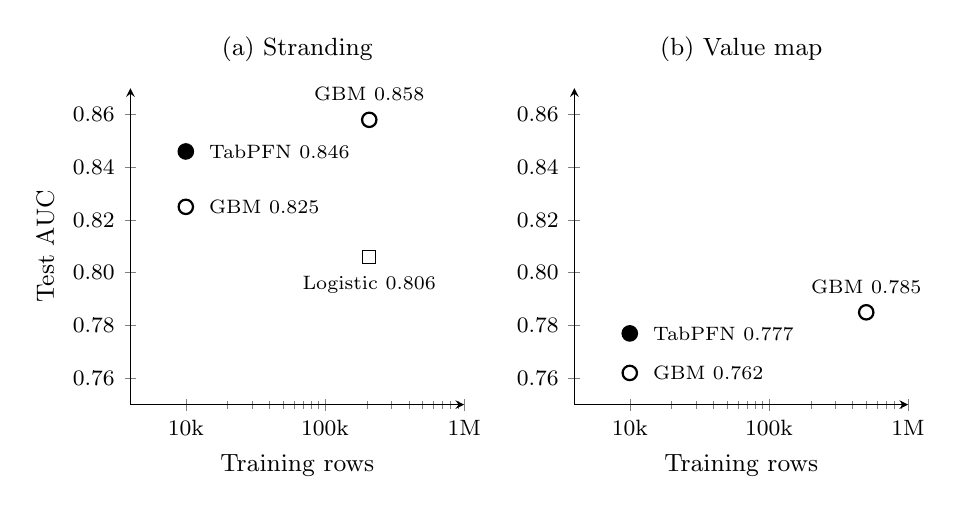
\begin{tikzpicture}
\begin{axis}[
  name=strand, width=0.48\textwidth, height=5.6cm,
  xmode=log, xmin=4000, xmax=1000000,
  ymin=0.75, ymax=0.87,
  xtick={10000,100000,1000000}, xticklabels={10k,100k,1M},
  ytick={0.76,0.78,0.80,0.82,0.84,0.86},
  yticklabel style={/pgf/number format/fixed,/pgf/number format/precision=2,/pgf/number format/fixed zerofill},
  xlabel={Training rows}, ylabel={Test AUC},
  title={\small (a) Stranding},
  tick label style={font=\footnotesize}, label style={font=\small},
  axis lines=left, clip=false]
\addplot[only marks, mark=o, mark size=2.6pt, thick] coordinates {(10000,0.825) (208000,0.858)};
\addplot[only marks, mark=*, mark size=2.8pt] coordinates {(10000,0.846)};
\addplot[only marks, mark=square, mark size=2.4pt] coordinates {(208000,0.806)};
\node[font=\scriptsize, anchor=west] at (axis cs:12500,0.846) {TabPFN 0.846};
\node[font=\scriptsize, anchor=west] at (axis cs:12500,0.825) {GBM 0.825};
\node[font=\scriptsize, anchor=south] at (axis cs:208000,0.8615) {GBM 0.858};
\node[font=\scriptsize, anchor=north] at (axis cs:208000,0.8025) {Logistic 0.806};
\end{axis}
\begin{axis}[
  at={(strand.east)}, anchor=west, xshift=1.4cm,
  width=0.48\textwidth, height=5.6cm,
  xmode=log, xmin=4000, xmax=1000000,
  ymin=0.75, ymax=0.87,
  xtick={10000,100000,1000000}, xticklabels={10k,100k,1M},
  ytick={0.76,0.78,0.80,0.82,0.84,0.86},
  yticklabel style={/pgf/number format/fixed,/pgf/number format/precision=2,/pgf/number format/fixed zerofill},
  xlabel={Training rows},
  title={\small (b) Value map},
  tick label style={font=\footnotesize}, label style={font=\small},
  axis lines=left, clip=false]
\addplot[only marks, mark=o, mark size=2.6pt, thick] coordinates {(10000,0.762) (500000,0.785)};
\addplot[only marks, mark=*, mark size=2.8pt] coordinates {(10000,0.777)};
\node[font=\scriptsize, anchor=west] at (axis cs:12500,0.777) {TabPFN 0.777};
\node[font=\scriptsize, anchor=west] at (axis cs:12500,0.762) {GBM 0.762};
\node[font=\scriptsize, anchor=south] at (axis cs:500000,0.7885) {GBM 0.785};
\end{axis}
\end{tikzpicture}
\caption{Test AUC by number of training rows. Filled circle: TabPFN (10k-row context, no tuning); open circles: GBM; square: logistic regression. Only measured points are drawn; nothing is interpolated. \emph{Data: MILES public vehicle endpoint, Berlin, June 2024 (ride ends for (a), hourly parked-car snapshots for (b)); train 3--16 June, test 17--22 June.}}
\label{fig:budget}
\end{figure}

\subsection{Cold start in a new city}

\begin{table}[h]
\centering
\caption{Stranding AUC in a new city by number of local training rides $n$. Rows (a) and (b) come from one run on the Prior Labs API; rows (c) and (d) from the committed script (\texttt{coldstart\_results\_off.csv}, mean over six cities and three seeds). \emph{Data: MILES public vehicle endpoint, June 2024.}}
\label{tab:cold}
\begin{tabular}{lccc}
\toprule
Model & $n=50$ & $n=200$ & $n=1000$ \\
\midrule
(a) \textbf{TabPFN}, Berlin + local rides as context & \textbf{0.665} & \textbf{0.688} & \textbf{0.710} \\
(b) Best GBM baseline, same run & $\approx$\,0.61 & not run & $\approx$\,0.65 \\
(c) GBM trained on Berlin only (transfer) & 0.649 & 0.647 & 0.655 \\
(d) GBM trained on local rides only & 0.554 & 0.588 & 0.603 \\
\bottomrule
\end{tabular}
\end{table}

With Berlin context and no training, TabPFN reaches 0.665 to 0.710 as local rides grow from 50 to 1,000; a Berlin-transfer GBM is flat at about 0.65, and a GBM trained on local rides alone stays below 0.61 (Table~\ref{tab:cold}, Figure~\ref{fig:cold}). TabPFN's margin over the transfer GBM is small at $n=50$ (about 0.02) and grows to about 0.06 at $n=1000$, because it can use the local rides and the transfer GBM cannot. Rows (a) and (c) come from different runs, so this comparison is indicative until both are rerun together. This is the situation an operator faces when entering a new city.

\begin{figure}[t]
\centering
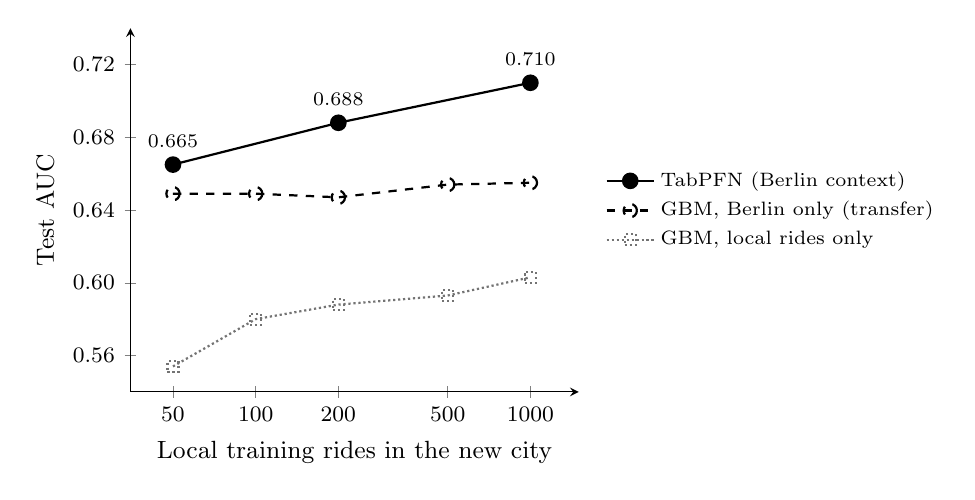
\begin{tikzpicture}
\begin{axis}[
  width=0.6\textwidth, height=6.2cm,
  xmode=log, xmin=35, xmax=1500,
  ymin=0.54, ymax=0.74,
  xtick={50,100,200,500,1000}, xticklabels={50,100,200,500,1000},
  ytick={0.56,0.60,0.64,0.68,0.72},
  yticklabel style={/pgf/number format/fixed,/pgf/number format/precision=2,/pgf/number format/fixed zerofill},
  xlabel={Local training rides in the new city}, ylabel={Test AUC},
  tick label style={font=\footnotesize}, label style={font=\small},
  axis lines=left, clip=false,
  legend style={font=\scriptsize, draw=none, at={(1.04,0.5)}, anchor=west}, legend cell align=left]
\addplot[mark=*, mark size=2.6pt, thick] coordinates {(50,0.665) (200,0.688) (1000,0.710)};
\addlegendentry{TabPFN (Berlin context)}
\addplot[mark=o, mark size=2.4pt, thick, dashed] coordinates {(50,0.649) (100,0.649) (200,0.647) (500,0.654) (1000,0.655)};
\addlegendentry{GBM, Berlin only (transfer)}
\addplot[mark=square, mark size=2.0pt, black!55, densely dotted, thick] coordinates {(50,0.554) (100,0.580) (200,0.588) (500,0.593) (1000,0.603)};
\addlegendentry{GBM, local rides only}
\node[font=\scriptsize, anchor=south] at (axis cs:50,0.669) {0.665};
\node[font=\scriptsize, anchor=south] at (axis cs:200,0.692) {0.688};
\node[font=\scriptsize, anchor=south] at (axis cs:1000,0.714) {0.710};
\end{axis}
\end{tikzpicture}
\caption{Cold start: stranding AUC in a new city by number of local rides. All lines connect measured points only. TabPFN: Prior Labs API run, measured at $n=50,200,1000$. GBM lines: committed script, mean over six cities and three seeds (\texttt{coldstart\_results\_off.csv}); they come from a different run than the TabPFN line. \emph{Data: MILES public vehicle endpoint, June 2024.}}
\label{fig:cold}
\end{figure}

\subsection{Value map: where to send the car}

The value map is trained on hourly snapshots of parked cars in Berlin, June 2024. The label is ``not rented within the next 12\,h'', and predictions are aggregated to 1\,km cells by hour.

\begin{table}[h]
\centering
\caption{Value map, $P(\text{not rented within 12\,h})$ for a parked car, test days. AUC is computed over parked-car snapshots; predictions are then averaged per 1\,km cell and hour for the map. \emph{Data: hourly fleet snapshots, MILES public vehicle endpoint, Berlin, June 2024.}}
\label{tab:value}
\begin{tabular}{lrc}
\toprule
Model & Training rows & AUC \\
\midrule
GBM & 10k & 0.762 \\
\textbf{TabPFN} & \textbf{10k} & \textbf{0.777} \\
GBM & 500k & 0.785 \\
\bottomrule
\end{tabular}
\end{table}

As for stranding, the full-data GBM leads, and TabPFN beats the GBM at equal data (Table~\ref{tab:value}). Per cell, predicted and observed rates correlate at $r = 0.90$. The map has strong structure in time and space. The share of cars not rented within 12\,h rises from 16\% for cars parked at 08--12\,h to 46\% at 20\,h, and from 7\% within 3\,km of the centre to 46\% beyond 15\,km.

\subsection{Still there when the rescuer arrives}

TabPFN predicts whether a flagged car is still available when a rescuer 5--30 minutes away arrives, with AUC 0.827. Calibration in the large is close: on the test days it predicts 4.7\% of cars gone, against 4.6\% observed. Same-budget GBM baselines for this task are pending and not reported here. If cars are shown only when $P(\text{still there}) \geq 95\%$, 68\% of flagged cars are shown and 1.2\% of rescues end with the car gone. With a \eur{5} credit refunded when the car is gone, the guarantee costs about \eur{6} per 100 rescues.

\subsection{Why cars strand}

\begin{table}[h]
\centering
\caption{Odds ratios for stranding, logistic regression on 208k Berlin ride ends. \emph{Data: MILES public vehicle endpoint, Berlin, training window 3--16 June 2024.}}
\label{tab:or}
\begin{tabular}{lr@{\hspace{2.5em}}lr}
\toprule
Factor & OR & Factor & OR \\
\midrule
Van & 5.5$\times$ & Fuel below 15\% & 1.5$\times$ \\
Ride ends 18--24\,h & 3.5$\times$ & Per 5\,km from centre & 1.3$\times$ \\
Large car & 3.1$\times$ & Electric & 0.8$\times$ \\
Premium & 2.5$\times$ & Per 100 departures nearby (24\,h) & 0.48$\times$ \\
Ride ends 00--06\,h & 1.7$\times$ & & \\
\bottomrule
\end{tabular}
\end{table}

Vehicle class and time of day dominate (Table~\ref{tab:or}). Local demand protects: 100 more departures nearby in the past day roughly halve the odds. Low fuel matters little, so stranding and refuelling are different problems. Stranded does not mean broken: 88\% of stranded waits end in a normal booking or ride, and 0.1\% in a repair. The value of a rescue is therefore time saved, not a rental that would otherwise never happen. The logistic model explains why cars strand; TabPFN ranks which car will strand, more accurately (AUC 0.846 against 0.806).

\section{Live deployment}\label{sec:live}

The stranding model is also served on current data. Live Berlin ride ends from our 2026 collector are micro-batched every 60\,s and sent to the Prior Labs TabPFN API, with the fixed June 2024 10k-row context. If a call times out (20\,s) or fails, that batch is scored by a GBM fallback instead. The counters are public at \url{https://miles.bolls.dev/ops/api/health}. Fetched \livets{}, cumulative since the service last restarted: \livecalls{} API calls, \liveok{} successful; \liverowstabpfn{} ride ends scored by TabPFN and \liverowsfallback{} by the fallback (\livefallbackbatches{} batches); median latency \livepfifty\,s per batch (90th percentile \livepninety\,s).

Three caveats apply. First, the served model uses a reduced feature set without the local supply and demand features; its out-of-sample AUC on 17--22 June 2024 ride ends is 0.822 (\texttt{miles-ops/model/tabpfn\_meta.json}), below the 0.846 of Table~\ref{tab:strand}. Second, the context is two years older than the ride ends it scores, and we have not yet evaluated live scores against realised outcomes. Third, the demo replay of June 2024 uses scores computed offline with the same context; it is labelled as replay.

\section{Economic scenarios}\label{sec:econ}

What a rescue programme is worth depends mainly on how many users accept an offer. We know of no published measurement for free-floating cars, so we give scenarios rather than one number.

The top 10\% of ride ends are flagged, about 1,490 per day, of which 58\% really strand (Table~\ref{tab:strand}). A rescue of a car that would have stranded is assumed to be worth \eur{17}--28 in recovered availability. The credit is \eur{5} and is paid for every accepted rescue, including the 42\% of flagged cars that would not have stranded. The annual value is
\begin{equation}
1{,}490 \times \text{acceptance} \times \left(0.58 \times \text{value of a rescue} - \text{\eur{5}}\right) \times 365.
\end{equation}

\begin{table}[h]
\centering
\caption{Annual recoverable value in Berlin by acceptance rate (value of a rescue \eur{17}--28, credit \eur{5}). Acceptance is unmeasured. \emph{Source: scenario model; inputs from Table~\ref{tab:strand} and stated assumptions.}}
\label{tab:econ}
\begin{tabular}{lcc}
\toprule
Acceptance & Rescues per day & Value per year \\
\midrule
5\% & $\approx$\,75 & \eur{130k}--300k \\
10\% & $\approx$\,150 & \eur{260k}--610k (central $\approx$\,\eur{0.4M}) \\
20\% & $\approx$\,300 & \eur{530k}--1.2M \\
\bottomrule
\end{tabular}
\end{table}

An alternative way to value the same rescues is avoided staff work: up to about \eur{1.3M} per year if accepted rescues replaced all of MILES' roughly 180 staff relocation trips per day ($180 \times \eur{20} \times 365$, with \eur{20} per trip assumed). This is not additive to Table~\ref{tab:econ}, and it needs about 12\% acceptance ($180 / 1{,}490$). Acceptance is defined per flagged car, so the still-there filter (68\% shown) and walking distance both reduce it. Stranded cars are mostly peripheral, which limits walk-up rescues (Section~\ref{sec:limits}).

\section{Proposed experiment: two weeks to measure acceptance}\label{sec:ab}

The economics hinge on one unmeasured number, so the next step is to measure it, not to model it further.
\begin{itemize}
\item \textbf{Unit.} A flagged opportunity: a ride end in the top 10\% of the stranding score, with positive net value and $P(\text{still there}) \geq 95\%$.
\item \textbf{Arms.} Randomize each opportunity 50/50 to \emph{offer} (\eur{5} credit, money back if gone) or \emph{holdout} (no offer). Optional extra arms at \eur{3} and \eur{8} estimate the price response.
\item \textbf{Duration.} Two weeks, so that both weekdays and weekends appear twice.
\item \textbf{Primary estimand.} Acceptance rate in the offer arm.
\item \textbf{Secondary estimands.} Intention-to-treat difference in the share of opportunities that strand and in mean idle hours, offer against holdout; net euros per opportunity; refund rate against the predicted 1.2\%.
\item \textbf{Size.} About 1,490 flagged ride ends per day give roughly 10,000 opportunities per arm in two weeks, before filtering. An illustrative power calculation: at 10\% acceptance, if a completed rescue lowers the stranding probability from 58\% to 20\%, the intention-to-treat difference is 3.8 percentage points, and detecting it at $\alpha = 0.05$ with 80\% power needs about 2,700 opportunities per arm. Clustering by area and day lowers the effective sample size, so standard errors should be clustered by cell and day.
\item \textbf{Pre-registration.} Arms, estimands and analysis are fixed before launch. Credits are paid only for completed rescues.
\end{itemize}

\section{Limitations}\label{sec:limits}

\begin{itemize}
\item \textbf{Historical data.} All model results come from one summer month in Berlin (June 2024), with a test window of six days. Seasonality is not modelled. The live service (Section~\ref{sec:live}) has not been evaluated against outcomes.
\item \textbf{GBM is more accurate on full Berlin data.} For stranding and the value map, the GBM trained on all data has the higher AUC, and for stranding also the lower ECE. TabPFN's advantages are cold start, data efficiency and calibration at equal data.
\item \textbf{Cold-start detail.} We report means without seed-level variance. The TabPFN row and the transfer-GBM row of Table~\ref{tab:cold} come from different runs. An earlier, smaller API run in the repository (two cities, two seeds, \texttt{coldstart\_results\_api.csv}) gave lower TabPFN cold-start AUCs (0.55--0.58); Table~\ref{tab:cold} reports the later rerun.
\item \textbf{Cannibalisation.} Moving a car adds supply to the target cell and can delay the next rental of cars already there. The value map does not model this. The intention-to-treat estimand of the experiment (Section~\ref{sec:ab}) measures the net effect, including this.
\item \textbf{Label.} $\mathit{idle\_h}$ measures time to the next status change of any kind, not strictly to the next rental.
\item \textbf{No user data.} The models cannot personalise. Who is near a car, and whether they would accept, is unknown until the experiment.
% 7.3 km median, ~75% beyond 5 km: miles-ops/analysis/rescue_stranded_validation.md
\item \textbf{Stranded cars are peripheral.} The median stranded car is 7.3\,km from the centre and about 75\% are beyond 5\,km. A short walk-up rescue is realistic only for the inner-city share; for the rest, the operator console, which targets staff trips a day earlier, carries more volume.
\item \textbf{Assumed economics.} The value of a rescue (\eur{17}--28), the staff-trip cost (\eur{20}) and the acceptance rates are assumptions.
\item \textbf{Relocation baseline.} The 180 trips per day and the 24.6\,h delay are inferred heuristically from the public record of status changes (see the repository), not from operator logs.
\end{itemize}

\section{Reproducibility and ethics}

Code for data processing, labelling, training, evaluation and figures is released under Apache-2.0 at \url{https://github.com/LinusBolls/miles-ahead}, together with both proof-of-concept surfaces, following the spirit of the NeurIPS reproducibility checklist~\citep{pineau2021reproducibility}. The split is strictly by time and no feature uses information from after the ride end. The data contain no personal data; they describe cars, places and times only, collected from a public endpoint. MILES did not take part in this work and has not endorsed it.

\bibliographystyle{unsrtnat}
\bibliography{refs}

\end{document}
